\documentclass{article} % Starts an article
\usepackage{tikz}
\usetikzlibrary{shapes.geometric, arrows, calc}
\usepackage[numbib]{tocbibind}
\tikzstyle{cool} = [rectangle, rounded corners, minimum width=3cm, minimum
height=1cm, text centered, draw=black, fill=gray!30, text width=3cm]
\tikzstyle{arrow} = [thick, ->, >=stealth]
\tikzstyle{line} = [thick, -, >=stealth]


\begin{document}



\tikzstyle{cool} = [rectangle, rounded corners, minimum width=3cm, minimum
height=1cm, text centered, draw=black, fill=gray!30, text width=3cm]
\tikzstyle{arrow} = [thick, ->, >=stealth]
\tikzstyle{line} = [thick, -, >=stealth]

\begin{figure}
    \centering
    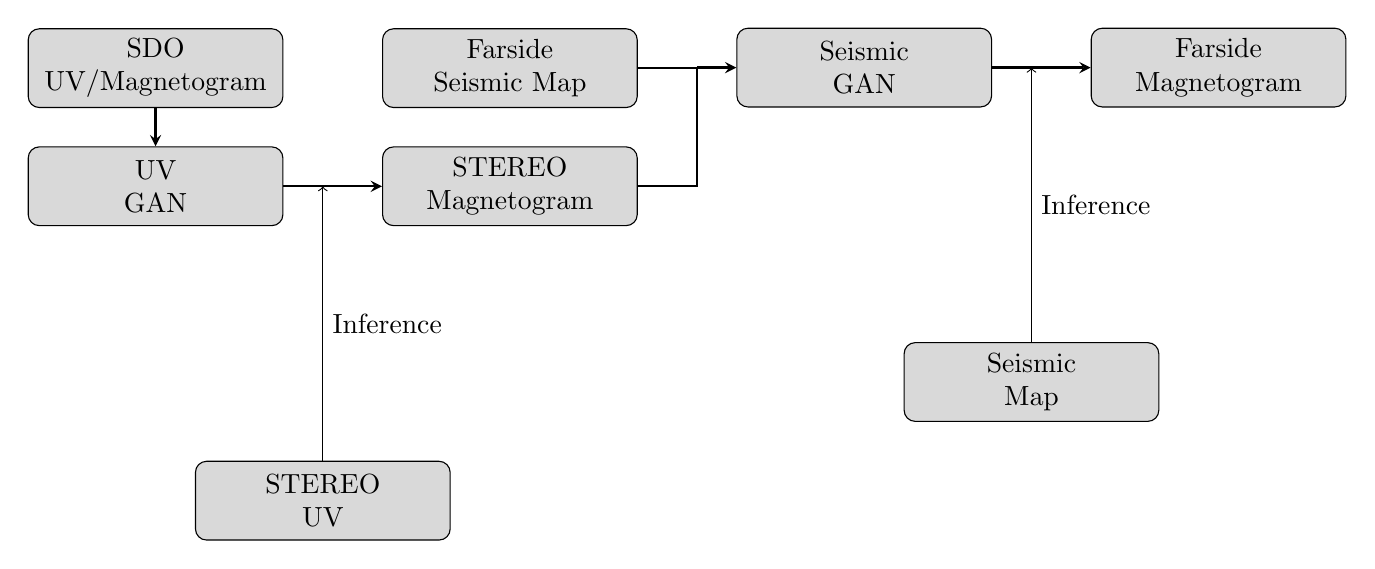
\begin{tikzpicture}[node distance=4.5cm]
        % \draw[help lines] (0,-5) grid (10,10);
        \node (SDO) [cool, above=1.5cm, left=1.5cm] {SDO\\ UV/Magnetogram};
        \node (UVGAN) [cool, left=1.5cm] {UV\\ GAN};
        \node (SM) [cool, right of=SDO] {Farside \quad \quad \quad \qquad  Seismic Map};
        % \node (E) [cool] {STEREO EUV image};
        \node (STEM) [cool, right of=UVGAN] {STEREO Magnetogram};
        \node (SGAN) [cool, right of=STEM, above=1cm] {Seismic\\ GAN};
        \node (FM) [cool, right of=SGAN] {Farside\\ Magnetogram};

        \coordinate (I1) at ([xshift=0.5cm]UVGAN.east); % we collect the edges in front of Q

        \node (SUV) [cool, below of=I1, above=0.0cm] {STEREO\\ UV};
        \draw [->] (SUV) -- node[anchor=west] {Inference} (I1);

        \coordinate (I2) at ([xshift=0.5cm]SGAN.east); % we collect the edges in front of Q

        \node (SM2) [cool, below of=I2, above=0.0cm] {Seismic\\ Map};
        \draw [->] (SM2) -- node[anchor=west] {Inference} (I2);

        \coordinate (T) at ([xshift=-0.5cm]SGAN.west);
        \draw [line] (STEM) -| (T);
        \draw [line] (SM) -| (T);
        \draw [arrow] (T) -> (SGAN);

        \draw [arrow] (SDO) -> (UVGAN);
        \draw [arrow] (UVGAN) -> (STEM);
        \draw [arrow] (SGAN) -> (FM);

        % \coordinate (FF) at ([xshift=-1.5cm]F.west); % we collect the edges in front of Q
        % \coordinate (MM) at ([xshift=-1.5cm]M.west); % we collect the edges in front of Q
        
        % \draw [arrow] (D) -- node[anchor=south, text width=2cm] {Helioseismic Holography} (P);
        % \draw [arrow] (MM) -- node[anchor=south] {cGAN} (M);
        % \draw [line] (P) -|  (FF);
        % \draw [line] (M) -|  (FF);
        % \draw [line] (S) -|  (MM);
        % % \draw [line] (E) -|  (MM);
        % \draw [arrow] (FF) -- node[anchor=south] {cGAN} (F);

    \end{tikzpicture}
    \caption{Test}
\end{figure}


\end{document}
